\documentclass[]{article}
\usepackage{lmodern}
\usepackage{amssymb,amsmath}
\usepackage{ifxetex,ifluatex}
\usepackage{fixltx2e} % provides \textsubscript
\ifnum 0\ifxetex 1\fi\ifluatex 1\fi=0 % if pdftex
  \usepackage[T1]{fontenc}
  \usepackage[utf8]{inputenc}
\else % if luatex or xelatex
  \ifxetex
    \usepackage{mathspec}
  \else
    \usepackage{fontspec}
  \fi
  \defaultfontfeatures{Ligatures=TeX,Scale=MatchLowercase}
\fi
% use upquote if available, for straight quotes in verbatim environments
\IfFileExists{upquote.sty}{\usepackage{upquote}}{}
% use microtype if available
\IfFileExists{microtype.sty}{%
\usepackage{microtype}
\UseMicrotypeSet[protrusion]{basicmath} % disable protrusion for tt fonts
}{}
\usepackage[margin=1in]{geometry}
\usepackage{hyperref}
\hypersetup{unicode=true,
            pdftitle={ragtop: Complex Derivatives Pricing},
            pdfauthor={Brian K. Boonstra},
            pdfborder={0 0 0},
            breaklinks=true}
\urlstyle{same}  % don't use monospace font for urls
\usepackage{color}
\usepackage{fancyvrb}
\newcommand{\VerbBar}{|}
\newcommand{\VERB}{\Verb[commandchars=\\\{\}]}
\DefineVerbatimEnvironment{Highlighting}{Verbatim}{commandchars=\\\{\}}
% Add ',fontsize=\small' for more characters per line
\usepackage{framed}
\definecolor{shadecolor}{RGB}{248,248,248}
\newenvironment{Shaded}{\begin{snugshade}}{\end{snugshade}}
\newcommand{\KeywordTok}[1]{\textcolor[rgb]{0.13,0.29,0.53}{\textbf{#1}}}
\newcommand{\DataTypeTok}[1]{\textcolor[rgb]{0.13,0.29,0.53}{#1}}
\newcommand{\DecValTok}[1]{\textcolor[rgb]{0.00,0.00,0.81}{#1}}
\newcommand{\BaseNTok}[1]{\textcolor[rgb]{0.00,0.00,0.81}{#1}}
\newcommand{\FloatTok}[1]{\textcolor[rgb]{0.00,0.00,0.81}{#1}}
\newcommand{\ConstantTok}[1]{\textcolor[rgb]{0.00,0.00,0.00}{#1}}
\newcommand{\CharTok}[1]{\textcolor[rgb]{0.31,0.60,0.02}{#1}}
\newcommand{\SpecialCharTok}[1]{\textcolor[rgb]{0.00,0.00,0.00}{#1}}
\newcommand{\StringTok}[1]{\textcolor[rgb]{0.31,0.60,0.02}{#1}}
\newcommand{\VerbatimStringTok}[1]{\textcolor[rgb]{0.31,0.60,0.02}{#1}}
\newcommand{\SpecialStringTok}[1]{\textcolor[rgb]{0.31,0.60,0.02}{#1}}
\newcommand{\ImportTok}[1]{#1}
\newcommand{\CommentTok}[1]{\textcolor[rgb]{0.56,0.35,0.01}{\textit{#1}}}
\newcommand{\DocumentationTok}[1]{\textcolor[rgb]{0.56,0.35,0.01}{\textbf{\textit{#1}}}}
\newcommand{\AnnotationTok}[1]{\textcolor[rgb]{0.56,0.35,0.01}{\textbf{\textit{#1}}}}
\newcommand{\CommentVarTok}[1]{\textcolor[rgb]{0.56,0.35,0.01}{\textbf{\textit{#1}}}}
\newcommand{\OtherTok}[1]{\textcolor[rgb]{0.56,0.35,0.01}{#1}}
\newcommand{\FunctionTok}[1]{\textcolor[rgb]{0.00,0.00,0.00}{#1}}
\newcommand{\VariableTok}[1]{\textcolor[rgb]{0.00,0.00,0.00}{#1}}
\newcommand{\ControlFlowTok}[1]{\textcolor[rgb]{0.13,0.29,0.53}{\textbf{#1}}}
\newcommand{\OperatorTok}[1]{\textcolor[rgb]{0.81,0.36,0.00}{\textbf{#1}}}
\newcommand{\BuiltInTok}[1]{#1}
\newcommand{\ExtensionTok}[1]{#1}
\newcommand{\PreprocessorTok}[1]{\textcolor[rgb]{0.56,0.35,0.01}{\textit{#1}}}
\newcommand{\AttributeTok}[1]{\textcolor[rgb]{0.77,0.63,0.00}{#1}}
\newcommand{\RegionMarkerTok}[1]{#1}
\newcommand{\InformationTok}[1]{\textcolor[rgb]{0.56,0.35,0.01}{\textbf{\textit{#1}}}}
\newcommand{\WarningTok}[1]{\textcolor[rgb]{0.56,0.35,0.01}{\textbf{\textit{#1}}}}
\newcommand{\AlertTok}[1]{\textcolor[rgb]{0.94,0.16,0.16}{#1}}
\newcommand{\ErrorTok}[1]{\textcolor[rgb]{0.64,0.00,0.00}{\textbf{#1}}}
\newcommand{\NormalTok}[1]{#1}
\usepackage{longtable,booktabs}
\usepackage{graphicx,grffile}
\makeatletter
\def\maxwidth{\ifdim\Gin@nat@width>\linewidth\linewidth\else\Gin@nat@width\fi}
\def\maxheight{\ifdim\Gin@nat@height>\textheight\textheight\else\Gin@nat@height\fi}
\makeatother
% Scale images if necessary, so that they will not overflow the page
% margins by default, and it is still possible to overwrite the defaults
% using explicit options in \includegraphics[width, height, ...]{}
\setkeys{Gin}{width=\maxwidth,height=\maxheight,keepaspectratio}
\IfFileExists{parskip.sty}{%
\usepackage{parskip}
}{% else
\setlength{\parindent}{0pt}
\setlength{\parskip}{6pt plus 2pt minus 1pt}
}
\setlength{\emergencystretch}{3em}  % prevent overfull lines
\providecommand{\tightlist}{%
  \setlength{\itemsep}{0pt}\setlength{\parskip}{0pt}}
\setcounter{secnumdepth}{0}
% Redefines (sub)paragraphs to behave more like sections
\ifx\paragraph\undefined\else
\let\oldparagraph\paragraph
\renewcommand{\paragraph}[1]{\oldparagraph{#1}\mbox{}}
\fi
\ifx\subparagraph\undefined\else
\let\oldsubparagraph\subparagraph
\renewcommand{\subparagraph}[1]{\oldsubparagraph{#1}\mbox{}}
\fi

%%% Use protect on footnotes to avoid problems with footnotes in titles
\let\rmarkdownfootnote\footnote%
\def\footnote{\protect\rmarkdownfootnote}

%%% Change title format to be more compact
\usepackage{titling}

% Create subtitle command for use in maketitle
\newcommand{\subtitle}[1]{
  \posttitle{
    \begin{center}\large#1\end{center}
    }
}

\setlength{\droptitle}{-2em}
  \title{ragtop: Complex Derivatives Pricing}
  \pretitle{\vspace{\droptitle}\centering\huge}
  \posttitle{\par}
  \author{Brian K. Boonstra}
  \preauthor{\centering\large\emph}
  \postauthor{\par}
  \predate{\centering\large\emph}
  \postdate{\par}
  \date{First Version: May 20, 2016 This Version: 2018-12-09}

\usepackage{amsmath}

\begin{document}
\maketitle

{
\setcounter{tocdepth}{2}
\tableofcontents
}
\subsection{Introduction}\label{introduction}

\textbf{ragtop} prices equity derivatives on variants of the famous
Black-Scholes model, with special attention paid to the case of American
and European exercise options and to convertible bonds. Convertible
bonds are one of the few types of derivative securities straddling asset
classes, and whose valuation must be linked to reasonable models of
\emph{multiple} asset types, involving equity valuations, fixed income
and sometimes foreign exchange.

A \textbf{convertible bond} is similar to a corporate bond\footnote{A
  standard corporate bond is often called a \emph{straight} bond},
promising coupons and notional payments at some known set of future
dates, but with a twist. The bond holder, who has effectively lent money
to the issuer, can choose to \emph{convert} the bond into equity
(subject to some restrictions), in a varying amount known as the
\emph{conversion value}. The bond value therefore depends on three major
processes:

\begin{itemize}
\tightlist
\item
  \emph{equity} value affecting conversion value
\item
  \emph{default} of the issuer wiping out equity, coupons and notional
\item
  \emph{interest rates} affecting the discounted value of future coupons
  and notional
\end{itemize}

Of these processes, the changes in equity value are most important,
followed closely by issuer default\footnote{One might wonder how a
  fixed-income security could be relatively insensitive to stochastic
  interest rates. Most convertibles are issued in countries with stable
  economies, so the rates are generally far less variable and far
  smaller than the credit spreads of the bond issuers.}. We perform
derivative pricing and calibration based on simply linked models of
equities and corporate defaults.

\subsection{Stochastic Model}\label{stochastic-model}

Our basic stochastic model links equity values \(S_t\) with \emph{hazard
rate} or default intensity \(h\) \[
    \frac{dS_t}{S_t}=(r+h-q) dt + \sigma dZ - dJ
\]

and can be converted to a PDE satisfied by any derivative of \(S\) that
lacks cashflows

\[
{{\frac{\partial \mspace{-1.0mu} V}{\partial \mspace{-1.0mu} t}}} -rV + h(\delta-V) + \left(r-q+h\right)S{{\frac{\partial \mspace{-1.0mu} V}{\partial \mspace{-1.0mu} S}}}+\frac12 \sigma^2 S^2 {{\frac{\partial^2 \mspace{-1.0mu} V}{\partial \mspace{-1.0mu} S^2}}}=0.
\]

\textbf{ragtop} numerically integrates this PDE using an implicit
scheme, forming solutions \(v^{(m)}_n\) on a grid of times
\(t^{(m)}, m=0,\dots,M\) and stock prices \(S_n, n=-N,\dots,N\). The
present value of our derivative is represented by the entry
\(v^{(M)}_0\).

For further details, please see the
\href{http://thureoscapital.com/ragtop.pdf}{technical paper}.

\subsection{Option Market Data}\label{option-market-data}

We have included some option market data in \textbf{ragtop}, consisting
of a set of several hundred option details for Tesla Motor in April
2016. This includes an underlying price

\begin{Shaded}
\begin{Highlighting}[]
\NormalTok{TSLAMarket}\OperatorTok{$}\NormalTok{S0}
\end{Highlighting}
\end{Shaded}

\begin{verbatim}
[1] 241.8
\end{verbatim}

A set of risk-free rates

\begin{Shaded}
\begin{Highlighting}[]
\NormalTok{knitr}\OperatorTok{::}\KeywordTok{kable}\NormalTok{(TSLAMarket}\OperatorTok{$}\NormalTok{risk_free_rates, }\DataTypeTok{digits=}\DecValTok{3}\NormalTok{, }\DataTypeTok{row.names =}\NormalTok{ F)}
\end{Highlighting}
\end{Shaded}

\begin{longtable}[]{@{}rr@{}}
\toprule
time & rate\tabularnewline
\midrule
\endhead
0.050 & 0.004\tabularnewline
0.127 & 0.005\tabularnewline
0.376 & 0.008\tabularnewline
0.625 & 0.010\tabularnewline
0.721 & 0.010\tabularnewline
1.718 & 0.010\tabularnewline
5.000 & 0.020\tabularnewline
\bottomrule
\end{longtable}

and some option price data, excerpted here:

\begin{longtable}[]{@{}rrrrrrr@{}}
\toprule
callput & K & time & mid & bid & ask & spread\tabularnewline
\midrule
\endhead
1 & 140 & 0.127 & 101.775 & 100.05 & 103.50 & 3.45\tabularnewline
-1 & 300 & 0.127 & 61.200 & 60.00 & 62.40 & 2.40\tabularnewline
1 & 360 & 0.376 & 1.745 & 1.57 & 1.92 & 0.35\tabularnewline
1 & 185 & 0.625 & 64.750 & 63.80 & 65.70 & 1.90\tabularnewline
-1 & 440 & 0.625 & 205.225 & 203.45 & 207.00 & 3.55\tabularnewline
-1 & 55 & 1.718 & 2.635 & 2.38 & 2.89 & 0.51\tabularnewline
\bottomrule
\end{longtable}

\subsection{Pricing Options}\label{pricing-options}

Tesla does not pay any dividends, so we can evaluate calls using the
Black Scholes model

\begin{verbatim}
$Price
[1] 69.47563

$Delta
[1] 0.8113372

$Vega
[1] 51.65849
\end{verbatim}

or better yet find the implied Black-Scholes volatility

\begin{Shaded}
\begin{Highlighting}[]
\KeywordTok{implied_volatility}\NormalTok{(}\DataTypeTok{option_price =}\NormalTok{ TSLAMarket}\OperatorTok{$}\NormalTok{options[}\DecValTok{400}\NormalTok{,}\StringTok{'ask'}\NormalTok{], }
                   \DataTypeTok{S0 =}\NormalTok{ TSLAMarket}\OperatorTok{$}\NormalTok{S0, }
                   \DataTypeTok{callput =}\NormalTok{ TSLAMarket}\OperatorTok{$}\NormalTok{options[}\DecValTok{400}\NormalTok{,}\StringTok{'callput'}\NormalTok{], }
                   \DataTypeTok{K=}\NormalTok{TSLAMarket}\OperatorTok{$}\NormalTok{options[}\DecValTok{400}\NormalTok{,}\StringTok{'K'}\NormalTok{], }
                   \DataTypeTok{r =} \FloatTok{0.005}\NormalTok{, }
                   \DataTypeTok{time =}\NormalTok{ TSLAMarket}\OperatorTok{$}\NormalTok{options[}\DecValTok{400}\NormalTok{,}\StringTok{'time'}\NormalTok{])}
\end{Highlighting}
\end{Shaded}

\begin{verbatim}
[1] 0.4151244
\end{verbatim}

For puts, we need to use a pricing algorithm that accounts for early
exercise. \textbf{ragtop} uses a control variate scheme on top of an
implicity PDE solver to achieve reasonable performance

\begin{Shaded}
\begin{Highlighting}[]
\KeywordTok{american}\NormalTok{(}
       \DataTypeTok{callput =}\NormalTok{ TSLAMarket}\OperatorTok{$}\NormalTok{options[}\DecValTok{400}\NormalTok{,}\StringTok{'callput'}\NormalTok{], }
       \DataTypeTok{S0 =}\NormalTok{ TSLAMarket}\OperatorTok{$}\NormalTok{S0, }
       \DataTypeTok{K=}\NormalTok{TSLAMarket}\OperatorTok{$}\NormalTok{options[}\DecValTok{400}\NormalTok{,}\StringTok{'K'}\NormalTok{], }
       \DataTypeTok{const_short_rate =} \FloatTok{0.005}\NormalTok{, }
       \DataTypeTok{time =}\NormalTok{ TSLAMarket}\OperatorTok{$}\NormalTok{options[}\DecValTok{400}\NormalTok{,}\StringTok{'time'}\NormalTok{])}
\end{Highlighting}
\end{Shaded}

\begin{verbatim}
A360_137_2 
  4.149565 
\end{verbatim}

This is also the underlying scheme for implied volatility

\begin{Shaded}
\begin{Highlighting}[]
\KeywordTok{american_implied_volatility}\NormalTok{(}\DataTypeTok{option_price =}\NormalTok{ TSLAMarket}\OperatorTok{$}\NormalTok{options[}\DecValTok{400}\NormalTok{,}\StringTok{'ask'}\NormalTok{], }
     \DataTypeTok{S0 =}\NormalTok{ TSLAMarket}\OperatorTok{$}\NormalTok{S0, }
     \DataTypeTok{callput =}\NormalTok{ TSLAMarket}\OperatorTok{$}\NormalTok{options[}\DecValTok{400}\NormalTok{,}\StringTok{'callput'}\NormalTok{], }
     \DataTypeTok{K=}\NormalTok{TSLAMarket}\OperatorTok{$}\NormalTok{options[}\DecValTok{400}\NormalTok{,}\StringTok{'K'}\NormalTok{], }
     \DataTypeTok{const_short_rate =} \FloatTok{0.005}\NormalTok{, }
     \DataTypeTok{time =}\NormalTok{ TSLAMarket}\OperatorTok{$}\NormalTok{options[}\DecValTok{400}\NormalTok{,}\StringTok{'time'}\NormalTok{])}
\end{Highlighting}
\end{Shaded}

\begin{verbatim}
[1] 0.415125
\end{verbatim}

\subsubsection{Including Default
Intensities}\label{including-default-intensities}

We can correct for constant intensities of default with parameters of
convenience, both for European exercise

\begin{Shaded}
\begin{Highlighting}[]
\KeywordTok{implied_volatility}\NormalTok{(}\DataTypeTok{option_price =} \DecValTok{17}\NormalTok{, }
                   \DataTypeTok{S0 =} \DecValTok{250}\NormalTok{, }\DataTypeTok{callput =}\NormalTok{ CALL,  }\DataTypeTok{K=}\DecValTok{245}\NormalTok{,}
                   \DataTypeTok{r =} \FloatTok{0.005}\NormalTok{, }\DataTypeTok{time =} \DecValTok{2}\NormalTok{,}
                   \DataTypeTok{const_default_intensity =} \FloatTok{0.03}\NormalTok{)}
\end{Highlighting}
\end{Shaded}

\begin{verbatim}
[1] NA
\end{verbatim}

and for American exercise

\begin{Shaded}
\begin{Highlighting}[]
\KeywordTok{american_implied_volatility}\NormalTok{(}\DataTypeTok{option_price =} \FloatTok{19.1}\NormalTok{, }
     \DataTypeTok{S0 =} \FloatTok{223.17}\NormalTok{, }\DataTypeTok{callput =}\NormalTok{ PUT, }\DataTypeTok{K=}\DecValTok{220}\NormalTok{, }
     \DataTypeTok{const_short_rate =} \FloatTok{0.005}\NormalTok{, }\DataTypeTok{time =} \FloatTok{1.45}\NormalTok{,}
     \DataTypeTok{const_default_intensity =} \FloatTok{0.0200}\NormalTok{)}
\end{Highlighting}
\end{Shaded}

\begin{verbatim}
[1] 0.1701377
\end{verbatim}

\subsubsection{Including Term
Structures}\label{including-term-structures}

If we have full term structures, we can use the associated parameters of
incovenience

\begin{Shaded}
\begin{Highlighting}[]
\NormalTok{## Dividends}
\NormalTok{divs =}\StringTok{ }\KeywordTok{data.frame}\NormalTok{(}\DataTypeTok{time=}\KeywordTok{seq}\NormalTok{(}\DataTypeTok{from=}\FloatTok{0.11}\NormalTok{, }\DataTypeTok{to=}\DecValTok{2}\NormalTok{, }\DataTypeTok{by=}\FloatTok{0.25}\NormalTok{),}
                  \DataTypeTok{fixed=}\KeywordTok{seq}\NormalTok{(}\FloatTok{1.5}\NormalTok{, }\DecValTok{1}\NormalTok{, }\DataTypeTok{length.out=}\DecValTok{8}\NormalTok{),}
                  \DataTypeTok{proportional =} \KeywordTok{seq}\NormalTok{(}\DecValTok{1}\NormalTok{, }\FloatTok{1.5}\NormalTok{, }\DataTypeTok{length.out=}\DecValTok{8}\NormalTok{))}

\NormalTok{## Interest rates}
\NormalTok{disct_fcn =}\StringTok{ }\NormalTok{ragtop}\OperatorTok{::}\KeywordTok{spot_to_df_fcn}\NormalTok{(}
  \KeywordTok{data.frame}\NormalTok{(}\DataTypeTok{time=}\KeywordTok{c}\NormalTok{(}\DecValTok{1}\NormalTok{, }\DecValTok{5}\NormalTok{, }\DecValTok{10}\NormalTok{, }\DecValTok{15}\NormalTok{),}
             \DataTypeTok{rate=}\KeywordTok{c}\NormalTok{(}\FloatTok{0.01}\NormalTok{, }\FloatTok{0.02}\NormalTok{, }\FloatTok{0.03}\NormalTok{, }\FloatTok{0.05}\NormalTok{))}
\NormalTok{)}

\NormalTok{## Default intensity}
\NormalTok{surv_prob_fcn =}\StringTok{ }\ControlFlowTok{function}\NormalTok{(T, t, ...) \{}
  \KeywordTok{exp}\NormalTok{(}\OperatorTok{-}\FloatTok{0.07} \OperatorTok{*}\StringTok{ }\NormalTok{(T }\OperatorTok{-}\StringTok{ }\NormalTok{t)) \}}

\NormalTok{## Variance cumulation / volatility term structure}
\NormalTok{vc =}\StringTok{ }\KeywordTok{variance_cumulation_from_vols}\NormalTok{(}
   \KeywordTok{data.frame}\NormalTok{(}\DataTypeTok{time=}\KeywordTok{c}\NormalTok{(}\FloatTok{0.1}\NormalTok{,}\DecValTok{2}\NormalTok{,}\DecValTok{3}\NormalTok{),}
              \DataTypeTok{volatility=}\KeywordTok{c}\NormalTok{(}\FloatTok{0.2}\NormalTok{,}\FloatTok{0.5}\NormalTok{,}\FloatTok{1.2}\NormalTok{)))}
\KeywordTok{paste0}\NormalTok{(}\StringTok{"Cumulated variance to 18 months is "}\NormalTok{, }\KeywordTok{vc}\NormalTok{(}\FloatTok{1.5}\NormalTok{, }\DecValTok{0}\NormalTok{))}
\end{Highlighting}
\end{Shaded}

\begin{verbatim}
[1] "Cumulated variance to 18 months is 0.369473684210526"
\end{verbatim}

to modify our estimates accordingly, including on vanilla option prices

\begin{Shaded}
\begin{Highlighting}[]
\KeywordTok{black_scholes_on_term_structures}\NormalTok{(}
   \DataTypeTok{callput=}\NormalTok{TSLAMarket}\OperatorTok{$}\NormalTok{options[}\DecValTok{500}\NormalTok{,}\StringTok{'callput'}\NormalTok{], }
   \DataTypeTok{S0=}\NormalTok{TSLAMarket}\OperatorTok{$}\NormalTok{S0, }
   \DataTypeTok{K=}\NormalTok{TSLAMarket}\OperatorTok{$}\NormalTok{options[}\DecValTok{500}\NormalTok{,}\StringTok{'K'}\NormalTok{], }
   \DataTypeTok{discount_factor_fcn=}\NormalTok{disct_fcn, }
   \DataTypeTok{time=}\NormalTok{TSLAMarket}\OperatorTok{$}\NormalTok{options[}\DecValTok{500}\NormalTok{,}\StringTok{'time'}\NormalTok{], }
   \DataTypeTok{survival_probability_fcn=}\NormalTok{surv_prob_fcn,}
   \DataTypeTok{variance_cumulation_fcn=}\NormalTok{vc,}
   \DataTypeTok{dividends=}\NormalTok{divs)}
\end{Highlighting}
\end{Shaded}

\begin{verbatim}
$Price
[1] 68.04663

$Delta
[1] 0.8289907

$Vega
[1] 47.06523
\end{verbatim}

American exercise option prices

\begin{Shaded}
\begin{Highlighting}[]
\KeywordTok{american}\NormalTok{(}
    \DataTypeTok{callput =}\NormalTok{ TSLAMarket}\OperatorTok{$}\NormalTok{options[}\DecValTok{400}\NormalTok{,}\StringTok{'callput'}\NormalTok{], }
    \DataTypeTok{S0 =}\NormalTok{ TSLAMarket}\OperatorTok{$}\NormalTok{S0, }
    \DataTypeTok{K=}\NormalTok{TSLAMarket}\OperatorTok{$}\NormalTok{options[}\DecValTok{400}\NormalTok{,}\StringTok{'K'}\NormalTok{], }
    \DataTypeTok{discount_factor_fcn=}\NormalTok{disct_fcn, }
    \DataTypeTok{time =}\NormalTok{ TSLAMarket}\OperatorTok{$}\NormalTok{options[}\DecValTok{400}\NormalTok{,}\StringTok{'time'}\NormalTok{],}
    \DataTypeTok{survival_probability_fcn=}\NormalTok{surv_prob_fcn,}
    \DataTypeTok{variance_cumulation_fcn=}\NormalTok{vc,}
    \DataTypeTok{dividends=}\NormalTok{divs)}
\end{Highlighting}
\end{Shaded}

\begin{verbatim}
A360_137_2 
  2.894296 
\end{verbatim}

and of course volatilities of European exercise options

\begin{Shaded}
\begin{Highlighting}[]
\KeywordTok{implied_volatility_with_term_struct}\NormalTok{(}
   \DataTypeTok{option_price =}\NormalTok{ TSLAMarket}\OperatorTok{$}\NormalTok{options[}\DecValTok{400}\NormalTok{,}\StringTok{'ask'}\NormalTok{], }
   \DataTypeTok{S0 =}\NormalTok{ TSLAMarket}\OperatorTok{$}\NormalTok{S0, }
   \DataTypeTok{callput =}\NormalTok{ TSLAMarket}\OperatorTok{$}\NormalTok{options[}\DecValTok{400}\NormalTok{,}\StringTok{'callput'}\NormalTok{], }
   \DataTypeTok{K=}\NormalTok{TSLAMarket}\OperatorTok{$}\NormalTok{options[}\DecValTok{400}\NormalTok{,}\StringTok{'K'}\NormalTok{], }
   \DataTypeTok{discount_factor_fcn=}\NormalTok{disct_fcn, }
   \DataTypeTok{time =}\NormalTok{ TSLAMarket}\OperatorTok{$}\NormalTok{options[}\DecValTok{400}\NormalTok{,}\StringTok{'time'}\NormalTok{],}
   \DataTypeTok{survival_probability_fcn=}\NormalTok{surv_prob_fcn,}
   \DataTypeTok{dividends=}\NormalTok{divs)}
\end{Highlighting}
\end{Shaded}

\begin{verbatim}
[1] 0.4112688
\end{verbatim}

as well as American exercise options

\begin{Shaded}
\begin{Highlighting}[]
\KeywordTok{american_implied_volatility}\NormalTok{(}
    \DataTypeTok{option_price=}\NormalTok{TSLAMarket}\OperatorTok{$}\NormalTok{options[}\DecValTok{400}\NormalTok{,}\StringTok{'ask'}\NormalTok{], }
    \DataTypeTok{callput =}\NormalTok{ TSLAMarket}\OperatorTok{$}\NormalTok{options[}\DecValTok{400}\NormalTok{,}\StringTok{'callput'}\NormalTok{], }
    \DataTypeTok{S0 =}\NormalTok{ TSLAMarket}\OperatorTok{$}\NormalTok{S0, }
    \DataTypeTok{K=}\NormalTok{TSLAMarket}\OperatorTok{$}\NormalTok{options[}\DecValTok{400}\NormalTok{,}\StringTok{'K'}\NormalTok{], }
    \DataTypeTok{discount_factor_fcn=}\NormalTok{disct_fcn, }
    \DataTypeTok{time =}\NormalTok{ TSLAMarket}\OperatorTok{$}\NormalTok{options[}\DecValTok{400}\NormalTok{,}\StringTok{'time'}\NormalTok{],}
    \DataTypeTok{survival_probability_fcn=}\NormalTok{surv_prob_fcn,}
    \DataTypeTok{dividends=}\NormalTok{divs)}
\end{Highlighting}
\end{Shaded}

\begin{verbatim}
[1] 0.4090605
\end{verbatim}

\subsection{Fitting Term Structures of
Volatility}\label{fitting-term-structures-of-volatility}

Let's say we have a some favored picture of our default intensity as a
function of stock price and time.

\begin{Shaded}
\begin{Highlighting}[]
\NormalTok{  def_ints_fcn =}\StringTok{ }\ControlFlowTok{function}\NormalTok{(t, S, ...)\{}
    \FloatTok{0.09}\OperatorTok{+}\FloatTok{0.01}\OperatorTok{*}\NormalTok{(S0}\OperatorTok{/}\NormalTok{S)}\OperatorTok{^}\FloatTok{1.5}
\NormalTok{    \}}
\end{Highlighting}
\end{Shaded}

Let's further postulate a set of financial instruments with known
prices. If those instruments all have different maturities, then
(generically) there is a unique piecewise constant volatility term
structure that will reproduce those prices.

\begin{Shaded}
\begin{Highlighting}[]
\NormalTok{  options_df =}\StringTok{ }\NormalTok{TSLAMarket}\OperatorTok{$}\NormalTok{options}
\NormalTok{  S0 =}\StringTok{ }\NormalTok{TSLAMarket}\OperatorTok{$}\NormalTok{S0}
\NormalTok{  make_option =}\StringTok{ }\ControlFlowTok{function}\NormalTok{(x) \{}
    \ControlFlowTok{if}\NormalTok{ (x[}\StringTok{'callput'}\NormalTok{]}\OperatorTok{>}\DecValTok{0}\NormalTok{) cp=}\StringTok{'C'} \ControlFlowTok{else}\NormalTok{ cp=}\StringTok{'P'}
\NormalTok{    ragtop}\OperatorTok{::}\KeywordTok{AmericanOption}\NormalTok{(}\DataTypeTok{callput=}\NormalTok{x[}\StringTok{'callput'}\NormalTok{], }\DataTypeTok{strike=}\NormalTok{x[}\StringTok{'K'}\NormalTok{], }\DataTypeTok{maturity=}\NormalTok{x[}\StringTok{'time'}\NormalTok{],}
                           \DataTypeTok{name=}\KeywordTok{paste}\NormalTok{(cp,x[}\StringTok{'K'}\NormalTok{],}\KeywordTok{as.integer}\NormalTok{(}\DecValTok{100}\OperatorTok{*}\NormalTok{x[}\StringTok{'time'}\NormalTok{]), }\DataTypeTok{sep=}\StringTok{'_'}\NormalTok{))}
\NormalTok{  \}}
\NormalTok{  atm_put_price =}\StringTok{ }\KeywordTok{max}\NormalTok{(options_df}\OperatorTok{$}\NormalTok{K[options_df}\OperatorTok{$}\NormalTok{K}\OperatorTok{<=}\NormalTok{S0])}
\NormalTok{  atm_put_ix =}\StringTok{ }\NormalTok{((options_df}\OperatorTok{$}\NormalTok{K}\OperatorTok{==}\NormalTok{atm_put_price) }\OperatorTok{&}\StringTok{ }\NormalTok{(options_df}\OperatorTok{$}\NormalTok{callput}\OperatorTok{==}\NormalTok{PUT)}
                \OperatorTok{&}\StringTok{ }\NormalTok{(options_df}\OperatorTok{$}\NormalTok{time}\OperatorTok{>}\DecValTok{1}\OperatorTok{/}\DecValTok{12}\NormalTok{))}
\NormalTok{  atm_puts =}\StringTok{ }\KeywordTok{apply}\NormalTok{(options_df[atm_put_ix,], }\DecValTok{1}\NormalTok{, make_option)}

\NormalTok{  atm_put_prices =}\StringTok{ }\NormalTok{options_df}\OperatorTok{$}\NormalTok{mid[atm_put_ix]}
\NormalTok{  knitr}\OperatorTok{::}\KeywordTok{kable}\NormalTok{(options_df[atm_put_ix,], }\DataTypeTok{digits=}\DecValTok{3}\NormalTok{, }\DataTypeTok{row.names =}\NormalTok{ F)}
\end{Highlighting}
\end{Shaded}

\begin{longtable}[]{@{}rrrrrrr@{}}
\toprule
callput & K & time & mid & bid & ask & spread\tabularnewline
\midrule
\endhead
-1 & 240 & 0.127 & 15.925 & 15.70 & 16.15 & 0.45\tabularnewline
-1 & 240 & 0.376 & 27.100 & 26.75 & 27.45 & 0.70\tabularnewline
-1 & 240 & 0.625 & 35.425 & 34.60 & 36.25 & 1.65\tabularnewline
-1 & 240 & 0.721 & 37.400 & 36.90 & 37.90 & 1.00\tabularnewline
-1 & 240 & 1.718 & 58.075 & 56.15 & 60.00 & 3.85\tabularnewline
\bottomrule
\end{longtable}

Once we have those instruments, we can successively fit our volatility
term structure to longer-and-longer dated securities. This is done for
us in the \texttt{fit\_variance\_cumulation} function

\begin{Shaded}
\begin{Highlighting}[]
\NormalTok{vcm =}\StringTok{ }\KeywordTok{fit_variance_cumulation}\NormalTok{(S0, }\DataTypeTok{eq_options=}\NormalTok{atm_puts,}
       \DataTypeTok{mid_prices=}\NormalTok{atm_put_prices,}
       \DataTypeTok{spreads=}\FloatTok{0.01}\OperatorTok{*}\NormalTok{atm_put_prices,}
       \DataTypeTok{use_impvol=}\OtherTok{TRUE}\NormalTok{,}
       \DataTypeTok{discount_factor_fcn=}\NormalTok{disct_fcn, }
       \DataTypeTok{default_intensity_fcn =}\NormalTok{ def_ints_fcn,}
       \DataTypeTok{num_time_steps=}\DecValTok{100}\NormalTok{)}
\NormalTok{vcm}\OperatorTok{$}\NormalTok{volatilities}
\end{Highlighting}
\end{Shaded}

\begin{verbatim}
[1] 0.4531763 0.4107467 0.3973169 0.3828557 0.3466839
\end{verbatim}

\subsection{Fitting Default Intensity}\label{fitting-default-intensity}

True default intensities are unobservable, even retrospectively, so it
is nearly impossible to form an historical time series of them. One may
try by using credit spreads, but even then an historical calibration may
be fairly unreliable for extension into the future. Our model requires
those future default intensities, so choosing a reasonable functional
form requires close attention. Our choice will generally arise from
fitting to available market information.

Since a full fit of the model requires calibration of both variance
cumulation and default intensity, our optimization algorithm must work
in two phases. It begins with a functional form of the user's choice,
such as

\[
h(S) = h_0 \left(  s+(1-s)  \left( \frac{S_0}{S} \right)^p  \right)
\]

and then takes a set of options, such as these

\begin{longtable}[]{@{}rrrrrrr@{}}
\toprule
callput & K & time & mid & bid & ask & spread\tabularnewline
\midrule
\endhead
-1 & 210 & 0.625 & 21.325 & 21.00 & 21.65 & 0.65\tabularnewline
-1 & 220 & 0.625 & 25.475 & 24.35 & 26.60 & 2.25\tabularnewline
-1 & 210 & 0.721 & 23.325 & 22.95 & 23.70 & 0.75\tabularnewline
-1 & 220 & 0.721 & 27.575 & 27.05 & 28.10 & 1.05\tabularnewline
-1 & 210 & 1.718 & 42.100 & 41.30 & 42.90 & 1.60\tabularnewline
-1 & 220 & 1.718 & 46.925 & 45.80 & 48.05 & 2.25\tabularnewline
\bottomrule
\end{longtable}

and tries to match their prices with the best possible choice of \(p\)
and \(s\), while still matching the volatility term structure as
required above.

To that end, we define an objective (or penalty) function comparing
instrument prices \(P_i\) to model prices \(\tilde{P}_i\)

\[
\pi(p,s) = \sum \left( \tilde{P}_i-\tilde{P}_i \right)^2
\]

\begin{Shaded}
\begin{Highlighting}[]
\NormalTok{  h0 =}\StringTok{ }\FloatTok{0.05}
\NormalTok{  fit_penalty =}\StringTok{ }\ControlFlowTok{function}\NormalTok{(p, s) \{}
\NormalTok{  def_intens_f =}\StringTok{ }\ControlFlowTok{function}\NormalTok{(t,S,...) \{h0 }\OperatorTok{*}\StringTok{ }\NormalTok{(s }\OperatorTok{+}\StringTok{ }\NormalTok{(}\DecValTok{1}\OperatorTok{-}\NormalTok{s) }\OperatorTok{*}\StringTok{ }\NormalTok{(S0}\OperatorTok{/}\NormalTok{S)}\OperatorTok{^}\NormalTok{p)\}}
\NormalTok{  varnce =}\StringTok{ }\KeywordTok{fit_variance_cumulation}\NormalTok{(}
\NormalTok{              S0, }\DataTypeTok{eq_options=}\NormalTok{atm_puts,}
              \DataTypeTok{mid_prices=}\NormalTok{atm_put_prices,}
              \DataTypeTok{spreads=}\FloatTok{0.01}\OperatorTok{*}\NormalTok{atm_put_prices,}
              \DataTypeTok{use_impvol=}\OtherTok{TRUE}\NormalTok{,}
              \DataTypeTok{default_intensity_fcn =}\NormalTok{ def_intens_f,}
              \DataTypeTok{discount_factor_fcn=}\NormalTok{disct_fcn, }
              \DataTypeTok{num_time_steps=}\DecValTok{100}\NormalTok{)}
\NormalTok{  pvs_list =}\StringTok{ }\KeywordTok{find_present_value}\NormalTok{(}
              \DataTypeTok{S0=}\NormalTok{S0, }\DataTypeTok{instruments=}\NormalTok{fit_targets,}
              \DataTypeTok{default_intensity_fcn=}\NormalTok{def_intens_f,}
              \DataTypeTok{variance_cumulation_fcn=}\NormalTok{varnce}\OperatorTok{$}\NormalTok{cumulation_function,}
              \DataTypeTok{discount_factor_fcn=}\NormalTok{disct_fcn,}
              \DataTypeTok{num_time_steps=}\DecValTok{45}\NormalTok{)}
\NormalTok{  pvs =}\StringTok{ }\KeywordTok{as.numeric}\NormalTok{(pvs_list)}
\NormalTok{  pensum =}\StringTok{ }\KeywordTok{sum}\NormalTok{((fit_target_prices }\OperatorTok{-}\StringTok{ }\NormalTok{pvs)}\OperatorTok{^}\DecValTok{2}\NormalTok{)}
\NormalTok{  pensum}
\NormalTok{\}}
\KeywordTok{fit_penalty}\NormalTok{(}\DecValTok{1}\NormalTok{, }\FloatTok{0.5}\NormalTok{)}
\end{Highlighting}
\end{Shaded}

\begin{verbatim}
[1] 7.918304
\end{verbatim}

We can apply our favorite optimizer to this penalty function in order to
optimize the model parameters. \textbf{ragtop} includes one such fitting
algorithm in \texttt{fit\_to\_option\_market} and its simpler but less
featureful companion \texttt{fit\_to\_option\_market\_df}. Let's say we
have decided \(h_0=0.04\), \(s=0.75\) and \(p=5/2\). We may have some
other instrument we wish to price consistent with this calibration, such
as a convertible bond

\begin{Shaded}
\begin{Highlighting}[]
\NormalTok{cb =}\StringTok{ }\NormalTok{ragtop}\OperatorTok{::}\KeywordTok{ConvertibleBond}\NormalTok{(}
  \DataTypeTok{maturity=}\FloatTok{2.87}\NormalTok{, }\DataTypeTok{conversion_ratio=}\FloatTok{2.7788}\NormalTok{, }\DataTypeTok{notional=}\DecValTok{1000}\NormalTok{,}
  \DataTypeTok{coupons=}\KeywordTok{data.frame}\NormalTok{(}\DataTypeTok{payment_time=}\KeywordTok{seq}\NormalTok{(}\FloatTok{2.8}\NormalTok{,}\DecValTok{0}\NormalTok{, }\DataTypeTok{by=}\OperatorTok{-}\FloatTok{0.25}\NormalTok{),}
                     \DataTypeTok{payment_size=}\DecValTok{1000}\OperatorTok{*}\FloatTok{0.0025}\OperatorTok{/}\DecValTok{4}\NormalTok{),}
  \DataTypeTok{discount_factor_fcn =}\NormalTok{ disct_fcn,}
  \DataTypeTok{name=}\StringTok{'CBond'}
\NormalTok{)}

\NormalTok{s =}\StringTok{ }\FloatTok{0.75}
\NormalTok{h0 =}\StringTok{ }\FloatTok{0.04}
\NormalTok{p =}\StringTok{ }\FloatTok{2.5}
\end{Highlighting}
\end{Shaded}

of course we then need to make sure we have set up the associated
variance accumulator function

\begin{Shaded}
\begin{Highlighting}[]
\NormalTok{calibrated_intensity_f =}\StringTok{ }\ControlFlowTok{function}\NormalTok{(t, S, ...)\{}
  \FloatTok{0.03}\OperatorTok{+}\FloatTok{0.01}\OperatorTok{*}\NormalTok{(S0}\OperatorTok{/}\NormalTok{S)}\OperatorTok{^}\FloatTok{1.5}
\NormalTok{\}}

\NormalTok{calib_varnce =}\StringTok{ }\KeywordTok{fit_variance_cumulation}\NormalTok{(}
\NormalTok{              S0, }\DataTypeTok{eq_options=}\NormalTok{atm_puts,}
              \DataTypeTok{mid_prices=}\NormalTok{atm_put_prices,}
              \DataTypeTok{spreads=}\FloatTok{0.01}\OperatorTok{*}\NormalTok{atm_put_prices,}
              \DataTypeTok{use_impvol=}\OtherTok{TRUE}\NormalTok{,}
              \DataTypeTok{default_intensity_fcn =}\NormalTok{ calibrated_intensity_f,}
              \DataTypeTok{discount_factor_fcn=}\NormalTok{disct_fcn, }
              \DataTypeTok{num_time_steps=}\DecValTok{100}\NormalTok{)}
\NormalTok{calib_varnce}\OperatorTok{$}\NormalTok{volatilities}
\end{Highlighting}
\end{Shaded}

\begin{verbatim}
[1] 0.4802569 0.4572752 0.4574770 0.4483994 0.4478110
\end{verbatim}

Now we simply need to run our pricing algorithm

\begin{Shaded}
\begin{Highlighting}[]
\NormalTok{cb_value =}\StringTok{ }\KeywordTok{form_present_value_grid}\NormalTok{(}
  \DataTypeTok{S0=}\NormalTok{S0, }\DataTypeTok{grid_center=}\NormalTok{S0,}
  \DataTypeTok{instruments=}\KeywordTok{list}\NormalTok{(}\DataTypeTok{Convertible=}\NormalTok{cb),}
  \DataTypeTok{num_time_steps=}\DecValTok{250}\NormalTok{,}
  \DataTypeTok{default_intensity_fcn=}\NormalTok{calibrated_intensity_f,}
  \DataTypeTok{discount_factor_fcn =}\NormalTok{ disct_fcn,}
  \DataTypeTok{variance_cumulation_fcn=}\NormalTok{calib_varnce}\OperatorTok{$}\NormalTok{cumulation_function)}
\end{Highlighting}
\end{Shaded}

For convenience, \textbf{ragtop} also exposes the full grid from its
solver, allowing us to calculate delta and gamma

\begin{Shaded}
\begin{Highlighting}[]
\NormalTok{cbprices =}\StringTok{ }\NormalTok{ragtop}\OperatorTok{::}\KeywordTok{form_present_value_grid}\NormalTok{(}
  \DataTypeTok{S0=}\NormalTok{S0, }\DataTypeTok{grid_center=}\NormalTok{S0,}
  \DataTypeTok{instruments=}\KeywordTok{list}\NormalTok{(}\DataTypeTok{Convertible=}\NormalTok{cb),}
  \DataTypeTok{num_time_steps=}\DecValTok{250}\NormalTok{,}
  \DataTypeTok{default_intensity_fcn=}\NormalTok{calibrated_intensity_f,}
  \DataTypeTok{discount_factor_fcn =}\NormalTok{ disct_fcn,}
  \DataTypeTok{variance_cumulation_fcn=}\NormalTok{calib_varnce}\OperatorTok{$}\NormalTok{cumulation_function,}
  \DataTypeTok{std_devs_width=}\DecValTok{5}\NormalTok{)}
\NormalTok{cbgrid =}\StringTok{ }\KeywordTok{na.omit}\NormalTok{(}\KeywordTok{as.data.frame}\NormalTok{(cbprices))}

\NormalTok{present_value_interp =}\StringTok{ }\KeywordTok{splinefun}\NormalTok{(}
  \DataTypeTok{x=}\NormalTok{cbgrid[,}\StringTok{"Underlying"}\NormalTok{],}
  \DataTypeTok{y=}\NormalTok{cbgrid[,}\StringTok{"Convertible"}\NormalTok{])}

\NormalTok{delta =}\StringTok{ }\KeywordTok{present_value_interp}\NormalTok{(S0, }\DataTypeTok{deriv=}\DecValTok{1}\NormalTok{)}
\NormalTok{delta}
\end{Highlighting}
\end{Shaded}

\begin{verbatim}
[1] 1.663418
\end{verbatim}

or to make a plot

\begin{Shaded}
\begin{Highlighting}[]
\NormalTok{present_value =}\StringTok{ }\KeywordTok{present_value_interp}\NormalTok{(S0)}
\NormalTok{cbplot =}\StringTok{ }\NormalTok{( }\KeywordTok{ggplot}\NormalTok{(cbgrid,}
                  \KeywordTok{aes}\NormalTok{(}\DataTypeTok{x=}\NormalTok{Underlying,}\DataTypeTok{y=}\NormalTok{Convertible)) }\OperatorTok{+}
\StringTok{             }\KeywordTok{geom_line}\NormalTok{(}\DataTypeTok{size=}\FloatTok{1.2}\NormalTok{) }\OperatorTok{+}
\StringTok{             }\KeywordTok{scale_x_continuous}\NormalTok{(}\DataTypeTok{limits=}\KeywordTok{c}\NormalTok{(}\DecValTok{0}\NormalTok{,}\FloatTok{2.5}\OperatorTok{*}\NormalTok{S0)) }\OperatorTok{+}
\StringTok{             }\KeywordTok{scale_y_continuous}\NormalTok{(}\DataTypeTok{limits=}\KeywordTok{c}\NormalTok{(}\DecValTok{0}\NormalTok{,}\FloatTok{2.5}\OperatorTok{*}\NormalTok{cb}\OperatorTok{$}\NormalTok{notional)) }\OperatorTok{+}
\StringTok{             }\KeywordTok{geom_point}\NormalTok{(}\KeywordTok{aes}\NormalTok{(}\DataTypeTok{x=}\NormalTok{S0,}\DataTypeTok{y=}\NormalTok{present_value), }\DataTypeTok{color=}\StringTok{"red"}\NormalTok{) }\OperatorTok{+}
\StringTok{             }\KeywordTok{labs}\NormalTok{(}\DataTypeTok{title=}\StringTok{"Convertible Bond Value"}\NormalTok{)}
\NormalTok{)}
\NormalTok{cbplot}
\end{Highlighting}
\end{Shaded}

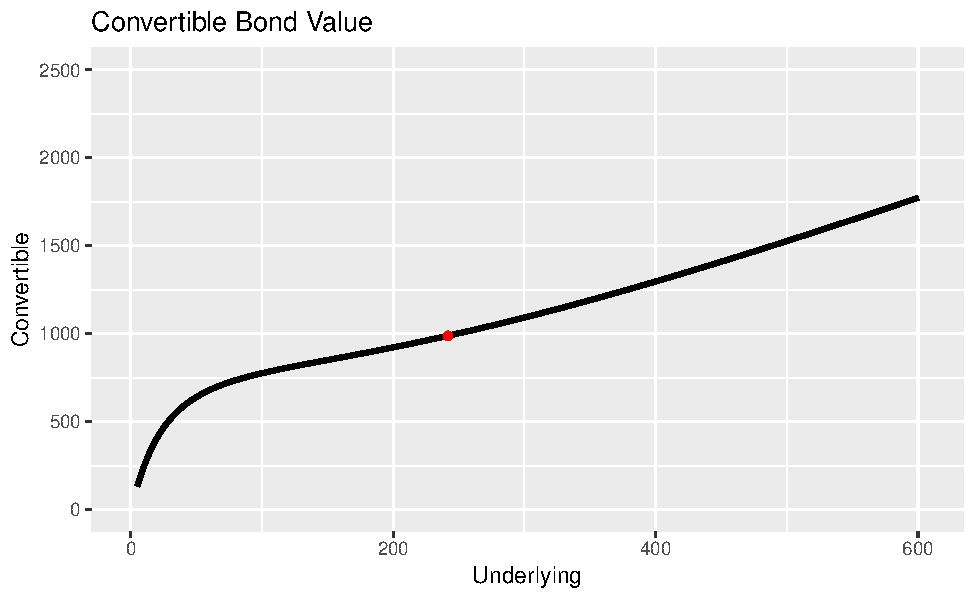
\includegraphics{Figs/grid_cb_plot-1.pdf}

\subsection{References}\label{references}


\end{document}
